\documentclass[10pt,a4paper]{article}
\usepackage[utf8]{inputenc}
\usepackage{amsmath}
\usepackage{amsfonts}
\usepackage{amssymb}
\usepackage{graphicx}

\begin{document}
Limit Definition: $\lim_{x\leftarrow a}{f(x)} = L$ if and only if $\lim_{x\leftarrow a^{-}}{f(x)} = L$ and $\lim_{x\leftarrow a^{+}}{f(x)} = L$
\\A vertical asymptote defined by the line $x=a$ is called a \textbf{vertical asymptote} of the function $f(x)$ if the both the left and right limit go to either $-\infty$ or $\infty$
\subsection{Limit Laws}
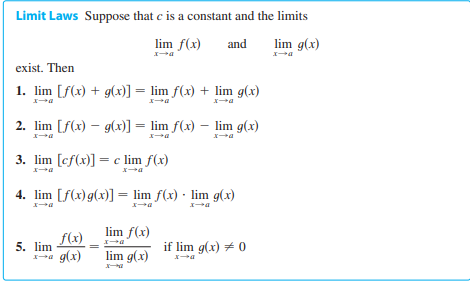
\includegraphics[scale=0.75]{limlaws}
Power law: $\lim_{x \rightarrow a}{[f(x)]^{n}}$ is equal to $[\lim_{x\rightarrow a}{f(x)}]^{n}$
\\$\lim_{x\rightarrow a}{x^{n}} = a^{n}$ where n is a  positive integer
\\Roots: $\lim_{x\rightarrow a}{\sqrt[n]{x}} = \sqrt[n]{a}$
\\Direct Substitution Property: If f is a polynomial or a rational function and a is in the domain of f then: $\lim{x\rightarrow a}{f(x)} = f(a)$
\\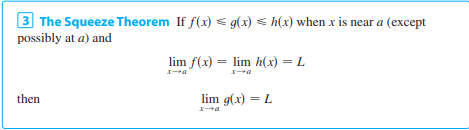
\includegraphics{squeeze}
\subsection{Precie Definition of a Limit}
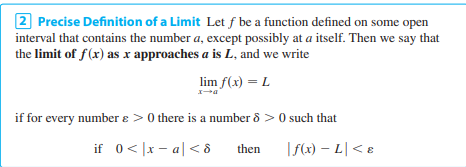
\includegraphics[scale=0.75]{preli}
\subsection{Continuity}
A function \textbf{f} is continuous at a number a if $\lim_{x \rightarrow a}{f(x)} = f(a)$
\\This means that 1. $f(a)$ is defined 2. $\lim_{x\rightarrow a}{f(x)} exists$  3. $lim{x \rightarrow a}{f(x)} = f(a)$
\\ \textbf{Definition:} A function f is continuous on an interval if it is continuous for every number in the interval
\\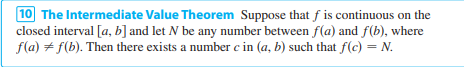
\includegraphics{ivt}
\subsection{Limits at infinity/Horizontal Asymptotes}
The line $y = L$ is called a horizontal aymptote of the curve $y=f(x)$ if either $\lim_{x\rightarrow \infty}{f(x)} = L$ or $\lim_{x\rightarrow -\infty}{f(x)} = L$
\\If $r > 0$ is a rational number then : $\lim{x\rightarrow \infty}{\frac{1}{x^{r}}}=0$
\\ If $r>0$ is a rational number such that $x^{r}$ is defined for all x then: $\lim_{x\rightarrow -\infty}{\frac{1}{x^{r}}} = 0$
\\ $\lim_{x \rightarrow -\infty}{e^{x}} = 0 $
\subsection{Derivatives and Rates of Change}
The tangent line to the curve $y=f(x)$ at the point $P(a,f(a))$ is the line through P with slope $m = \lim{x \rightarrow a}{\frac{f(x)-f(a)}{x-a}}$ provided the limit exists
\\\textbf{LIMIT DEFINITION OF A FUNCTION}: $f'(a) = \lim{h\rightarrow a}{\frac{f(a+h)-f(a)}{h}}$
\\Instantaneous rate of change: $\lim_{\delta x \rightarrow 0}{\frac{\delta y}{\delta x}} = \lim{x_{2}\rightarrow x_{1}}{\frac{f(x_{2})-f(x_{1})}{x_{2} - x_{1}}}$
\\\textbf{FUNCTIONS CAN BE CONTINUOUS AND DIFFERENTIABLE BUT NOT DIFFERENTIABLE AND CONTINUOUS}
\subsection{Derivation Rules}
Derivative of a constant: $\frac{d}{dx}(x) = 1$
\\Power Rule: $\frac{d}{dx}(x^{n}) = nx^{n-1}$
\\Constant Multiple Rule: $\frac{d}{dx}[cf(x)] = c\frac{d}{dx}f(x)$
\\Sum Rule: $\frac{d}{dx}[f(x)+g(x)] = \frac{d}{dx}f(x)+\frac{d}{dx}g(x)$
\\Difference Rule: $\frac{d}{dx}[f(x)-g(x)] = \frac{d}{dx}f(x)-\frac{d}{dx}g(x)$
\\Definition of the Number e: e is a number such that $ \lim_{h \rightarrow 0}{\frac{e^{h}-1}{h}}=1$ as such the derivative of $e^{x} is e^{x}$
\\When taking the derivative of $e^{nx}$ the derivative will become $ne^{nx}$
\\Product Rule: If f and g are both differentiable then: $\frac{d}{dx}[f(x)g(x)] = f(x)\frac{d}{dx}[g(x)]+g(x)\frac{d}{dx}[f(x)]$
\\Quotient Rule: If f and g are both differentiable then: $\frac{d}{dx}{\frac{f(x)}{dx}} = \frac{g(x)\frac{d}{dx}[f(x)]-f(x)\frac{d}{dx}[g(x)]}{[g(x)]^{2}}$
\\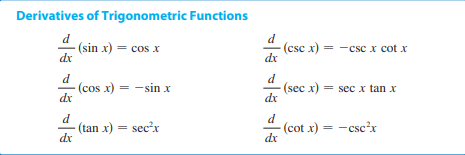
\includegraphics[scale=0.75]{trigder}
\end{document}